% !TeX program = xelatex 
\documentclass{hitreport}

% 此处添加自己需要的package
% \usepackage{package}

% =============================================
% Part 0 封面基本信息
% =============================================

\title{课程\&实验报告} % 题目,可以使用 \\ 命令分行
\expname{实验一} % 实验题目
\college{计算学部} % 学院
\major{计算机科学与技术} % 专业
\classnum{1803105} % 班号
\stuid{学号} % 学号
\name{姓名} % 姓名
\labloc{格物207} % 实验地点
\instructor{指导教师} % 指导教师
\term{2020秋季学期} % 学期
\date{\today} % 实验日期,可以使用文字填写

\begin{document}

% =============================================
% Part 1 Header
% =============================================

% 制作封面 
\maketitle
% 摘要和关键字,如果不需要摘要,可将\begin{abstract}和\end{abstract}及二者之间内容注释,或去掉
\begin{abstract}
hitreport是为哈尔滨工业大学本科生制作的\LaTeX 模板。

\keywords{关键字\quad   \LaTeX \quad  report template}
\end{abstract}

% 制作目录
\tableofcontents
\newpage


% =============================================
% Part 2 Main document
% =============================================

\section{实验目标和内容}

\subsection{实验目标}
\begin{enumerate}
\item 掌握图像直方图概念,直方图均衡化,规定化;
\item 掌握图像同态滤波。
\end{enumerate}

\subsection{实验内容}
\begin{enumerate}
\item 实现图像直方图均衡化,规定化。显示并保存前、后直方图,均衡化、规定化后结果图像;
\item 实现同态滤波,显示并保存结果图像;
\item (选做)实现双边滤波,显示并保存结果图像。
\end{enumerate}

\section{实验环境}

\begin{enumerate}
\item Anaconda 4.8.4
\item Python 3.7.4
\item PyCharm 2019.1 (Professional Edition)
\item Windows 10 2004
\end{enumerate}

\section{实验原理}

\subsection{直方图均衡化}\label{sec:junhenghua}

假设灰度值最初是连续的,令变量\textit{r}表示待处理图像的灰度。假设\textit{r}的值域是$\left[0,L-1\right]$,$r=0$表示黑色,$r=L-1$表示白色。对于满足条件的\textit{r},做如下的线性变换(灰度映射):
\begin{align}
s=T\left(r\right),\quad 0\le r\le L-1
\end{align}
对输入图像中给定的灰度值\textit{r},将产生一个输出灰度值\textit{s}。

令$p_r\left(r\right)$和$p_s\left(s\right)$表示两幅不同图像中灰度值r和s的PDF(概率密度函数)。由概率论的基本结论可知,若已知$p_r\left(r\right)$和T$\left(r\right)$,且$T\left(r\right)$是连续的且在$\left[0,L-1\right]$上是可微的,则变换后的变量\textit{s}的PDF为
\begin{align}\label{equ:pss}
p_s\left(s\right)=p_r\left(r\right)\Big|\frac{\mathrm{d}r}{\mathrm{d}s}\Big|.
\end{align}
因此,我们知道输出灰度变量\textit{s}的PDF是由输入灰度的PDF和所用的变换函数决定的。

使用如下的变换函数
\begin{align}\label{equ:trans}
s=T\left(r\right)=\left(L-1\right)\varint\nolimits_{0}^{r}p_r\left(w\right)\mathrm{d}w.
\end{align}

我们使用式(\ref{equ:pss})求变换后的$p_s\left(s\right)$,根据莱布尼茨积分法则可知,
\begin{align}
\frac{\mathrm{d}s}{\mathrm{d}r} = \frac{\mathrm{d} T\left(r\right)}{\mathrm{d}r} = \left(L-1\right)\frac{\mathrm{d}}{\mathrm{d}r}\Big[\varint\nolimits_{0}^{r}p_r\left(w\right)\mathrm{d}w\Big] = \left(L-1\right)p_r\left(r\right).
\end{align}

用这个结果代替式(\ref{equ:pss})中的$\left. \mathrm{d}r/\mathrm{d}s \right.$,则有
\begin{align}
p_s\left(s\right)=p_r\left(r\right)\Big|\frac{\mathrm{d}r}{\mathrm{d}s}\Big| = p_r\left(r\right)\Big|\frac{1}{\left(L-1\right)p_r\left(r\right)}\Big| = \frac{1}{L-1},\quad 0\le s\le L-1
\end{align}
因此,执行了式(\ref{equ:trans})的灰度变换后,将产生一个均匀的PDF表征。

对于离散值,采用概率与求和来代替概率密度函数与积分,则式(\ref{equ:trans})中变换的离散形式为
\begin{align}\label{equ:skTrk}
s_k = T\left(r_k\right) = \left(L-1\right) \sum_{j=0}^{k}p_r\left(r_j\right),\quad k=0,1,2,\cdots,L-1
\end{align}
使用式(\ref{equ:skTrk})将输入图像中灰度级为$r_k$的每个像素映射为输出图像中灰度级为$s_k$的对应像素,得到处理后的图像。这就是直方图的均衡化。

\subsection{直方图规定化}\label{sec:guidinghua}

直方图规定化是一种生存具有规定直方图的图像的方法。考虑连续灰度\textit{r}和\textit{z},将它们当成PDF分别为$p_r\left(r\right)$何$p_z\left(z\right)$的随机变量来处理。其中,\textit{r}和\textit{z}分别表示为输入图像和输出图像的灰度级。

采用与式(\ref{equ:trans})相同的变换函数,定义关于变量\textit{z}的一个函数\textit{G},有如下性质:
\begin{align}\label{equ:Gz}
G\left(z\right) = \left(L-1\right)\varint\nolimits_{0}^{z}p_z\left(v\right)\mathrm{d}v = s,
\end{align}
式中,\textit{v}是积分假变量。可以证明$G\left(z\right) = s = T\left(r\right)$,因此\textit{z}必须满足条件
\begin{align}
z = G^{-1}\left(s\right) = G^{-1}\left[T\left(r\right)\right]
\end{align}
使用输入图像算出$p_r\left(r\right)$后,就可以使用式(\ref{equ:trans})得到变换函数$T\left(r\right)$。类似地,函数$G\left(z\right)$可以由式(\ref{equ:Gz})得到。

对于离散化的形式,采用如式(\ref{equ:skTrk})的直方图均衡化变换。类似地,给定一个规定值$s_k$,式(\ref{equ:Gz})的离散形式包括对一个\textit{q}值计算变换函数
\begin{align}
G\left(z_q\right) = \left(L-1\right)\sum_{i=1}^{z}p_z\left(z_i\right)
\end{align}
以便有
\begin{align}
G\left(z_q\right) = s_k
\end{align}
式中,$p_z\left(z_i\right)$是规定直方图的第\textit{i}个值。最后,由反变换得到希望的值$z_q$:
\begin{align}
z_q = G^{-1}\left(s_k\right)
\end{align}
对所有像素执行上述运算时,即从直方图均衡化后的图像中的\textit{s}值到输出图像中对应\textit{z}值的一个映射。这就是直方图的规定化。

\subsection{同态滤波}\label{sec:tongtai}

图像$f\left(x,y\right)$可以表示为其照射分量$i\left(x,y\right)$和反射分量$r\left(x,y\right)$的乘积,即
\begin{align}
f\left(x,y\right) = i\left(x,y\right)r\left(x,y\right)
\end{align}
为此,定义
\begin{align}
z\left(x,y\right) = \ln f\left(x,y\right) = \ln i\left(x,y\right) + \ln r\left(x,y\right)
\end{align}
则有
\begin{align}
\mathscr{F}\left[z\left(x,y\right)\right] = \mathscr{F}\left[\ln f\left(x,y\right)\right] = \mathscr{F}\left[\ln i\left(x,y\right)\right] + \mathscr{F}\left[r\left(x,y\right)\right]
\end{align}
或
\begin{align}
Z\left(u,v\right) = F_i\left(u,v\right) + F_r\left(u,v\right)
\end{align}
式中,$F_i\left(u,v\right)$和$F_r\left(u,v\right)$分别为$\ln i\left(x,y\right)$与$\ln r\left(x,y\right)$的傅里叶变换。

使用滤波器传递函数$H\left(u,v\right)$对$Z\left(u,v\right)$滤波,有
\begin{align}
S\left(u,v\right) = H\left(u,v\right)Z\left(u,v\right) = H\left(u,v\right)F_i\left(u,v\right) + H\left(u,v\right)F_r\left(u,v\right)
\end{align}
空域下滤波后的图像为
\begin{align}\label{equ:sxy}
s\left(x,y\right) = \mathscr{F}^{-1}\left[S\left(u,v\right)\right] = \mathscr{F}^{-1}\left[H\left(u,v\right)F_i\left(u,v\right)\right] + \mathscr{F}^{-1}\left[H\left(u,v\right)F_r\left(u,v\right)\right]
\end{align}

由定义
\begin{align}
i'\left(x,y\right) = \mathscr{F}^{-1}\left[H\left(u,v\right)F_i\left(u,v\right)\right]
\end{align}
和
\begin{align}
r'\left(x,y\right) = \mathscr{F}^{-1}\left[H\left(u,v\right)F_r\left(u,v\right)\right]
\end{align}
可以将式(\ref{equ:sxy})写为
\begin{align}
s\left(x,y\right) = i'\left(x,y\right) + r'\left(x,y\right)
\end{align}

最后,由于$z\left(x,y\right)$是通过取输入图像的自然对数形成的,可以通过将滤波后的结果取指数得到输出图像:
\begin{align}
g\left(x,y\right) = e^{s\left(x,y\right)} = e^{i'\left(x,y\right)}e^{r'\left(x,y\right)} = i_0\left(x,y\right)r_0\left(x,y\right)
\end{align}
式中,
\begin{align}
i_0\left(x,y\right) = e^{i'\left(x,y\right)}
\end{align}
和
\begin{align}
r_0\left(x,y\right) = e^{r'\left(x,y\right)}
\end{align}
是输出图像的照射分量和反射分量。

使用同态滤波器可以更好的控制照射分量和反射分量,规定滤波器传递函数$H\left(u,v\right)$以不同的控制方法来影响傅里叶变换的低频和高频分量。若选择$\gamma_L$和$\gamma_H$满足$\gamma_L<1$且$\gamma_H\ge 1$,则图\ref{fig:F}中的滤波器函数将衰减低频(照射)分量,放大高频(反射)分量,最终的结果是同时进行动态范围的压缩和对比度增强。

\begin{figure}[H]
\centering
\begin{tikzpicture}
\draw [<->] (0,5) node [left] {$H\left(u,v\right)$} -- (0,0)
node [below left] {} -- (8,0) node [below] {$D\left(u,v\right)$};

\draw [ultra thick, dashed] (0,1) node [left] {$\gamma_L$}  (0,3) node [left] {$\gamma_H$};

\draw [blue,thick] (0,1) parabola (1.5,2) parabola[bend at end] (3,3);
\draw [blue,thick] (3,3) -- (7,3);
\draw [black,thick, dashed] (0,3) -- (3,3) ;


\end{tikzpicture}
\caption{同态滤波器传递函数的径向剖面图}\label{fig:F}
\end{figure}


图\ref{fig:F}所示的函数形状可以用高通滤波器传递函数近似,采用如式(\ref{equ:Huv})的同态滤波传递函数。
\begin{align}\label{equ:Huv}
H\left(u,v\right) = \left(\gamma_H-\gamma_L\right)\Big[1-e^{\left. -cD^2\left(u,v\right)/D_0^2 \right.}\Big] + \gamma_L
\end{align}
式中,
\begin{align}
D\left(u,v\right) = \Big[\left(u-\left.P/2\right.\right)^2 + \left(v-\left.Q/2\right.\right)^2\Big]^{\left.1/2\right.}
\end{align}
$D_0$是一个正常数,$D\left(u,v\right)$表示频率域中点$\left(u,v\right)$到$P\times Q$频率矩形中心的距离,在$\gamma_L$和$\gamma_H$之间的过渡的常数\textit{c}控制函数的偏斜度。

式(\ref{equ:Huv})即所需要的频域下的同态滤波传递函数。


\subsection{双边滤波}\label{sec:shuangbian}

高斯滤波是最常用的图像去噪方法之一,它能很好地滤除掉图像中随机出现的高斯噪声,但是在实验一中我们知道,高斯滤波是一种低通滤波,它在滤除图像中噪声信号的同时,也会对图像中的边缘信息进行平滑,表现出来的结果就是图像变得模糊,是因为它在滤波过程中只关注了位置信息。即在滤波窗口内,距离中心点越近的点的权重越大;这种只关注距离的思想在某些情况下是可行的,例如在平坦的区域,距离越近的区域其像素分布也越相近,自然地,这些点的像素值对滤波中心点的像素值更有参考价值。但是在像素值出现跃变的边缘区域,这种方法会适得其反,损失掉有用的边缘信息。此时就出现了一类算法——边缘保护滤波方法,双边滤波就是最常用的边缘保护滤波方法。

双边滤波在高斯滤波的基础上加入了像素值权重项,也就是说既要考虑距离因素,也要考虑像素值差异的影响,像素值越相近,权重越大。

双边滤波器中,输出像素的值依赖于邻域像素的值的加权组合,设$g\left(x,y\right)$为输出图像,$f\left(x,y\right)$为输入图像,则
\begin{align}
g\left(x,y\right) = \frac{\sum_{k,l} f\left(k,l\right)w\left(i,j,k,l\right)}{\sum_{k,l}w\left(i,j,k,l\right)},
\end{align}
其中,权重系数$w\left(i,j,k,l\right)$取决于定义域核
\begin{align}
d\left(i,j,k,l\right) = \exp \left\{-\frac{\left(i-k\right)^2+\left(j-l\right)^2}{2\sigma_d^2}\right\}
\end{align}
和值域核
\begin{align}
r\left(i,j,k,l\right) = \exp \left\{-\frac{\lVert f\left(i,j\right) - f\left(k,l\right) \rVert^2}{2\sigma_r^2}\right\}
\end{align}
的乘积。即
\begin{align}
w\left(i,j,k,l\right) = \exp \left\{-\frac{\left(i-k\right)^2+\left(j-l\right)^2}{2\sigma_d^2}-\frac{\lVert f\left(i,j\right) - f\left(k,l\right) \rVert^2}{2\sigma_r^2}\right\}
\end{align}

也由此可见,双边滤波同时考虑了空间域与值域的差别。

\section{实验步骤}

实验中所有代码在附录可见。

\subsection{直方图均衡化}\label{sec:junhenghua1}

直方图均衡化的第一步是统计原图像中的各灰度值的概率分布,代码如下:
\begin{lstlisting}[language=python]
def generate_histogram(self):
    height, width = np.shape(self.img)
    for i in range(height):
        for j in range(width):
            # print(self.img[i, j])
            self.histogram[self.img[i, j]] += 1
    self.histogram = self.histogram / np.sum(self.histogram)
    return self.histogram
\end{lstlisting}

读取灰度范围较小的lena图片,实现章节\ref{sec:junhenghua}的算法对原图片进行直方图均衡化,最后调用matplotlib的pyplot库对均衡化前后两图片的频率分布直方图进行绘制。

直方图均衡化的核心代码如下:
\begin{lstlisting}[language=python]
def histogram_equalization(self):
	self.histogram_equal = np.cumsum(self.img_histogram)
    height, width = np.shape(self.img)
    self.histogram_equal = np.uint8(255 * self.histogram_equal + 0.5)
    out_image = np.uint8(np.zeros((height, width)))
    for i in range(height):
        for j in range(width):
            out_image[i, j] = self.histogram_equal[self.img[i, j]]
    cv.imshow("histogram equalization", out_image)
    cv.waitKey(0)
    cv.destroyAllWindows()
    write_img_to_file(out_image, 'histogram_result/histogram equalization of source image')
    histogram = Histogram(out_image)
    chart = histogram.generate_histogram()
    histogram.show_histogram("histogram equalization of source image", '../data/histogram_result/',
                             "histogram equalization of source image")
\end{lstlisting}

\subsection{直方图规定化}\label{sec:guidinghua1}

直方图规定化需要分别将模板图片和待规定化图片进行直方图均衡化,再计算由待规定化图片直方图到模板图片的直方图的反向映射。计算直方图均衡化的结果可以调用章节\ref{sec:junhenghua1},计算反向映射的核心代码如下:
\begin{lstlisting}[language=python]
def calculate_reverse_mapping(histogram):
    mapping = list(histogram)
    off_mapping = []
    pre_f = 0.0
    for i in range(256):
        try:
            temp_f = mapping.index(i)
            pre_f = temp_f
        except ValueError:
            temp_f = pre_f
        off_mapping.append(temp_f)
    off_mapping = np.array(off_mapping)
    # plt.bar(range(len(off_mapping)), off_mapping, width=1)
    # plt.title("reverse mapping")
    # plt.show()
    return off_mapping

def calculate_target_mapping(target_histogram, template_histogram):
    target_map = list(target_histogram)
    template_map = list(template_histogram)
    final_map = []
    for i in range(256):
        temp_tar = target_map[i]
        temp_tem = template_map[temp_tar]
        final_map.append(temp_tem)
    final_map = np.array(final_map)
    return final_map
\end{lstlisting}

分别对图片的RGB三通道进行直方图规定化,再组合到一起形成规定化之后的图片。

\subsection{同态滤波}\label{sec:tongtailv}

实现章节\ref{sec:tongtai}的同态滤波算法,对于式(\ref{equ:Huv})的同态滤波传递函数采用参数$\gamma_L=0.3$,$\gamma_H = 1.5$,$c=1$,$D_0=10$,进行同态滤波。

同态滤波需要将图片的照射分量和反射分量分别进行傅里叶变换,傅里叶变换与傅里叶反变换的代码见附录\ref{app:fft},同态滤波的详细步骤见附录\ref{app:homo}。


\subsection{双边滤波}

实现章节\ref{sec:shuangbian}的双边滤波算法,双边滤波器的滤波核的构造以及滤波过程,核心代码如下:

\begin{lstlisting}[language=python]
def generate_gauss_filter_template(self):
    color_coe = -0.5 / np.square(self.color_sigma)
    for i in range(256):
        self.color_weight.append(np.exp(i ** 2 * color_coe))
    space_coe = -0.5 / np.square(self.s_sigma)
    for i in range(-self.radius, self.radius + 1):
        for j in range(-self.radius, self.radius + 1):
            r_sq = np.exp((np.square(i) + np.square(j)) * space_coe)
            self.weight_s_x.append(i)
            self.weight_s_y.append(j)
            self.weight_s.append(r_sq)
            self.k_max += 1

def bilateral_filter_main(self, img):
    for i in range(self.height):
        for j in range(self.width):
            value = 0
            weight = 0
            for index in range(self.k_max):
                print("i, j, index ", i, j, index)
                temp_x = self.weight_s_x[index] + i
                temp_y = self.weight_s_y[index] + j
                if temp_x >= self.height or temp_y >= self.width or temp_x < 0 or temp_y < 0:
                    val = 0
                else:
                    val = img[temp_x][temp_y]
                temp_w = np.float32(self.weight_s[index]) * np.float32(self.color_weight[np.abs(val - img[i][j])])
                value += val * temp_w
                weight += temp_w
            img[i][j] = np.uint8(value / weight)
    return img

\end{lstlisting}

分别对彩色图片的RGB三个通道进行双边滤波,得到最后结果。

\section{实验结果}

\subsection{直方图均衡化}

选用一张灰度值不均衡的lena图片进行直方图均衡化。原图如图(\ref{fig:lenasource})所示,原图的直方图如图(\ref{fig:lenahistogram})所示,进行直方图均衡化后,均衡化之后的图片如图(\ref{fig:lenafilter})所示,均衡化后图片的直方图如图(\ref{fig:lenafilterhistogram})所示。

\begin{figure}[htb]
	\centering
	\subfloat[灰度值不均衡lena图]{
		\label{fig:lenasource}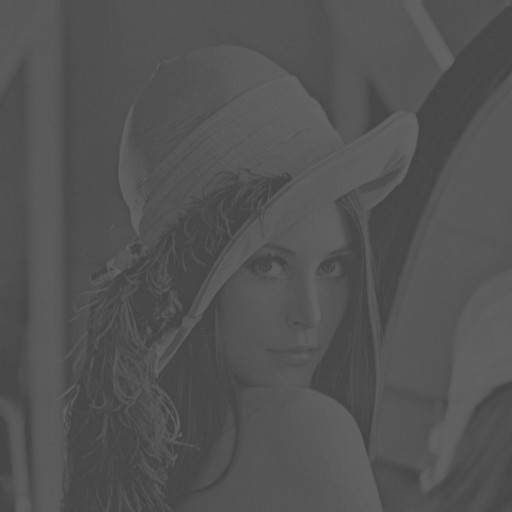
\includegraphics[width=.4\textwidth]{lenagray.jpg}}\hspace{20pt}
	\subfloat[灰度值不均衡lena图的直方图]{
		\label{fig:lenahistogram}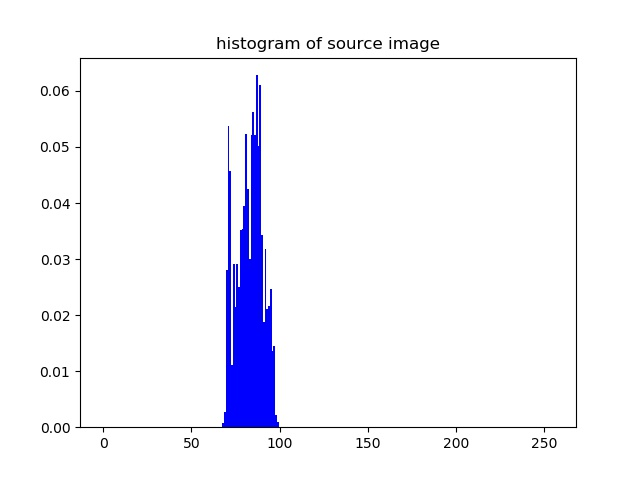
\includegraphics[width=.5\textwidth]{histogramofsourceimage.jpg}}
	\caption{灰度值不均衡lena图及其直方图}\label{fig:lena}
\end{figure}

\begin{figure}[htb]
	\centering
	\subfloat[直方图均衡化后的lena图]{
		\label{fig:lenafilter}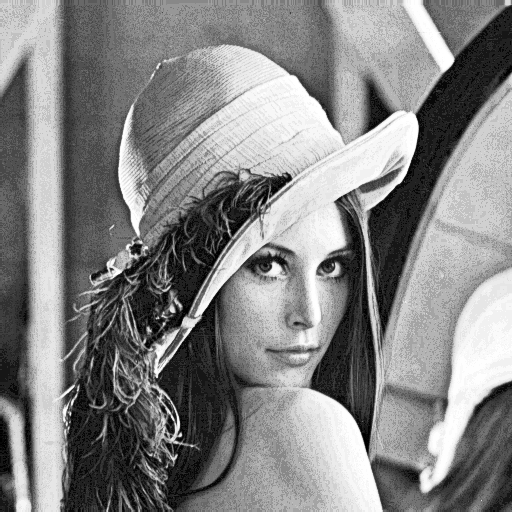
\includegraphics[width=.4\textwidth]{histogramequalizationofsourceimage.png}}\hspace{20pt}
	\subfloat[直方图均衡化后的lena图的直方图]{
		\label{fig:lenafilterhistogram}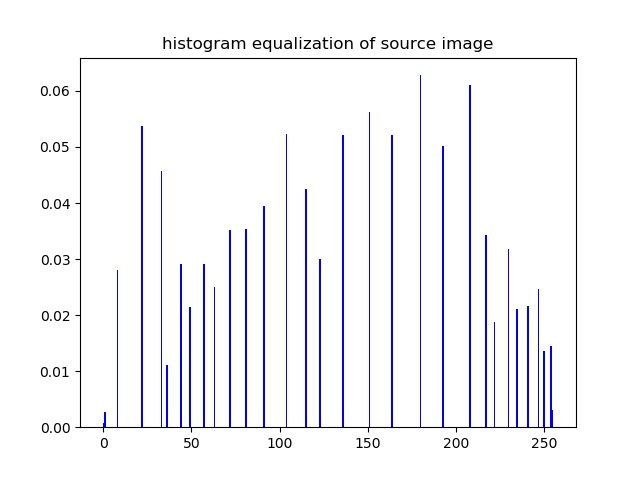
\includegraphics[width=.5\textwidth]{histogramequalizationofsourceimage.jpg}}
	\caption{直方图均衡化后的lena图及其直方图}\label{fig:lenafilter1}
\end{figure}


\subsection{直方图规定化}

直方图规定化选用的模板图片如图(\ref{fig:template})所示,其彩色直方图如图(\ref{fig:templatehistogram})所示。实现章节\ref{sec:guidinghua1}的算法。

\begin{figure}[htb]
	\centering
	\subfloat[模板图片]{
		\label{fig:template}
\includegraphics[width=.4\textwidth]{template.jpg}}\hspace{20pt}
	\subfloat[模板图片的彩色分布直方图]{
		\label{fig:templatehistogram}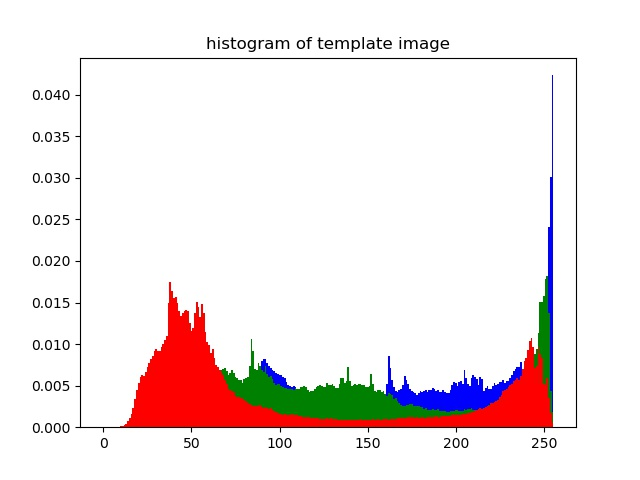
\includegraphics[width=.4\textwidth]{histogramoftemplateimage.jpg}}
	\caption{直方图规定化的模板图片及其彩色分布直方图}\label{fig:template1}
\end{figure}

选用的三幅待规定化图片及其彩色分布直方图如图(\ref{fig:guidinghua})所示。

\begin{figure}[htb]
	\centering
	\subfloat[待规定化图片1]{
		\label{fig:1}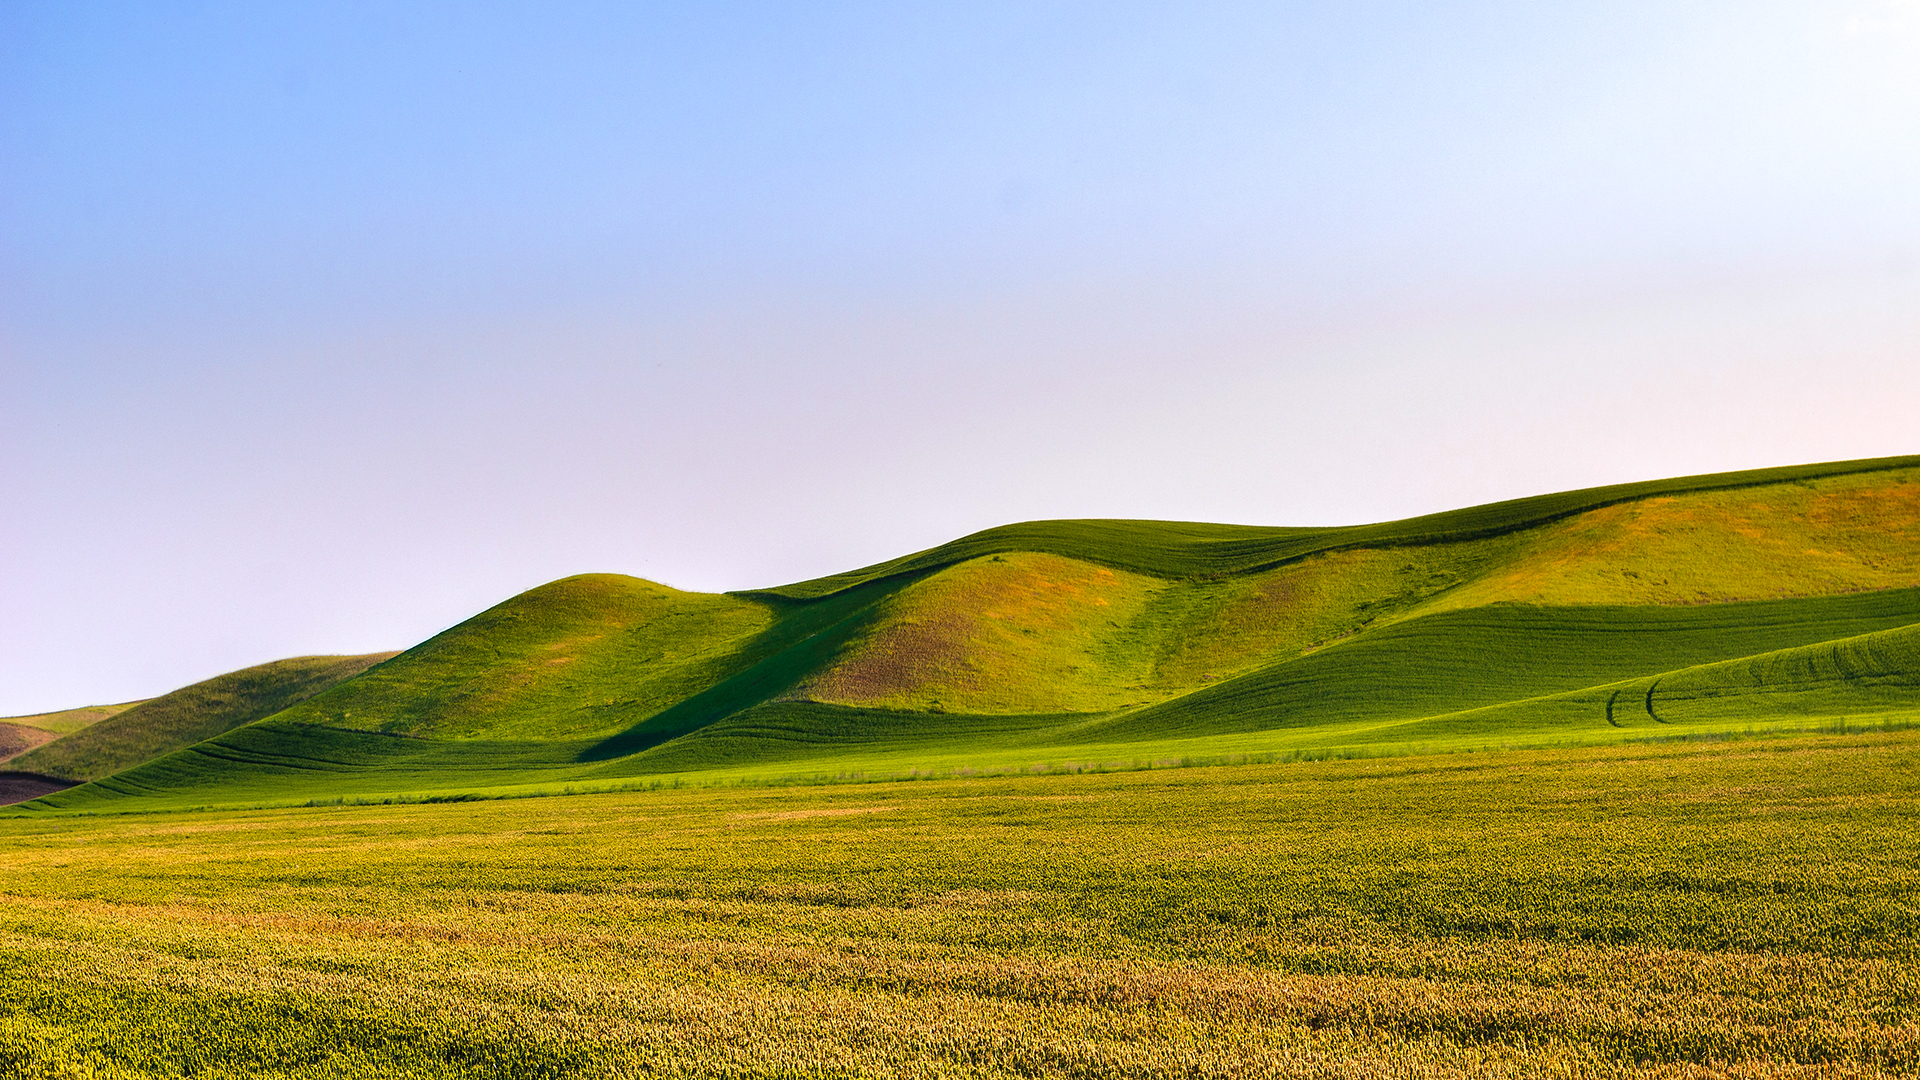
\includegraphics[width=.4\textwidth]{template1.jpg}}\hspace{20pt}
	\subfloat[待规定化图片1的彩色分布直方图]{
		\label{fig:1histogram}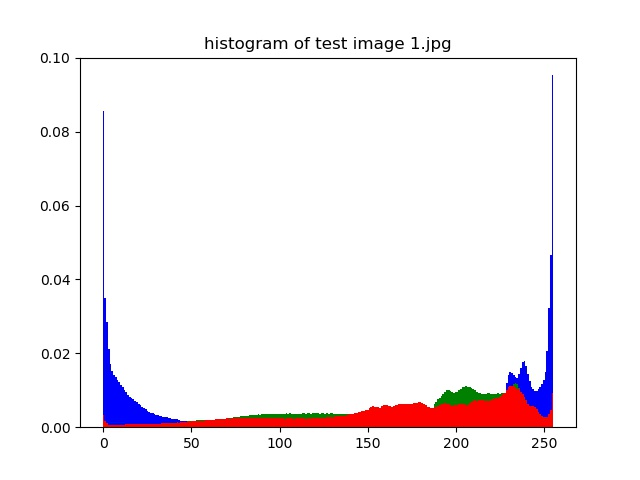
\includegraphics[scale=.3]{histogramoftestimage1.jpg}}
	\\
	\subfloat[待规定化图片2]{
		\label{fig:2}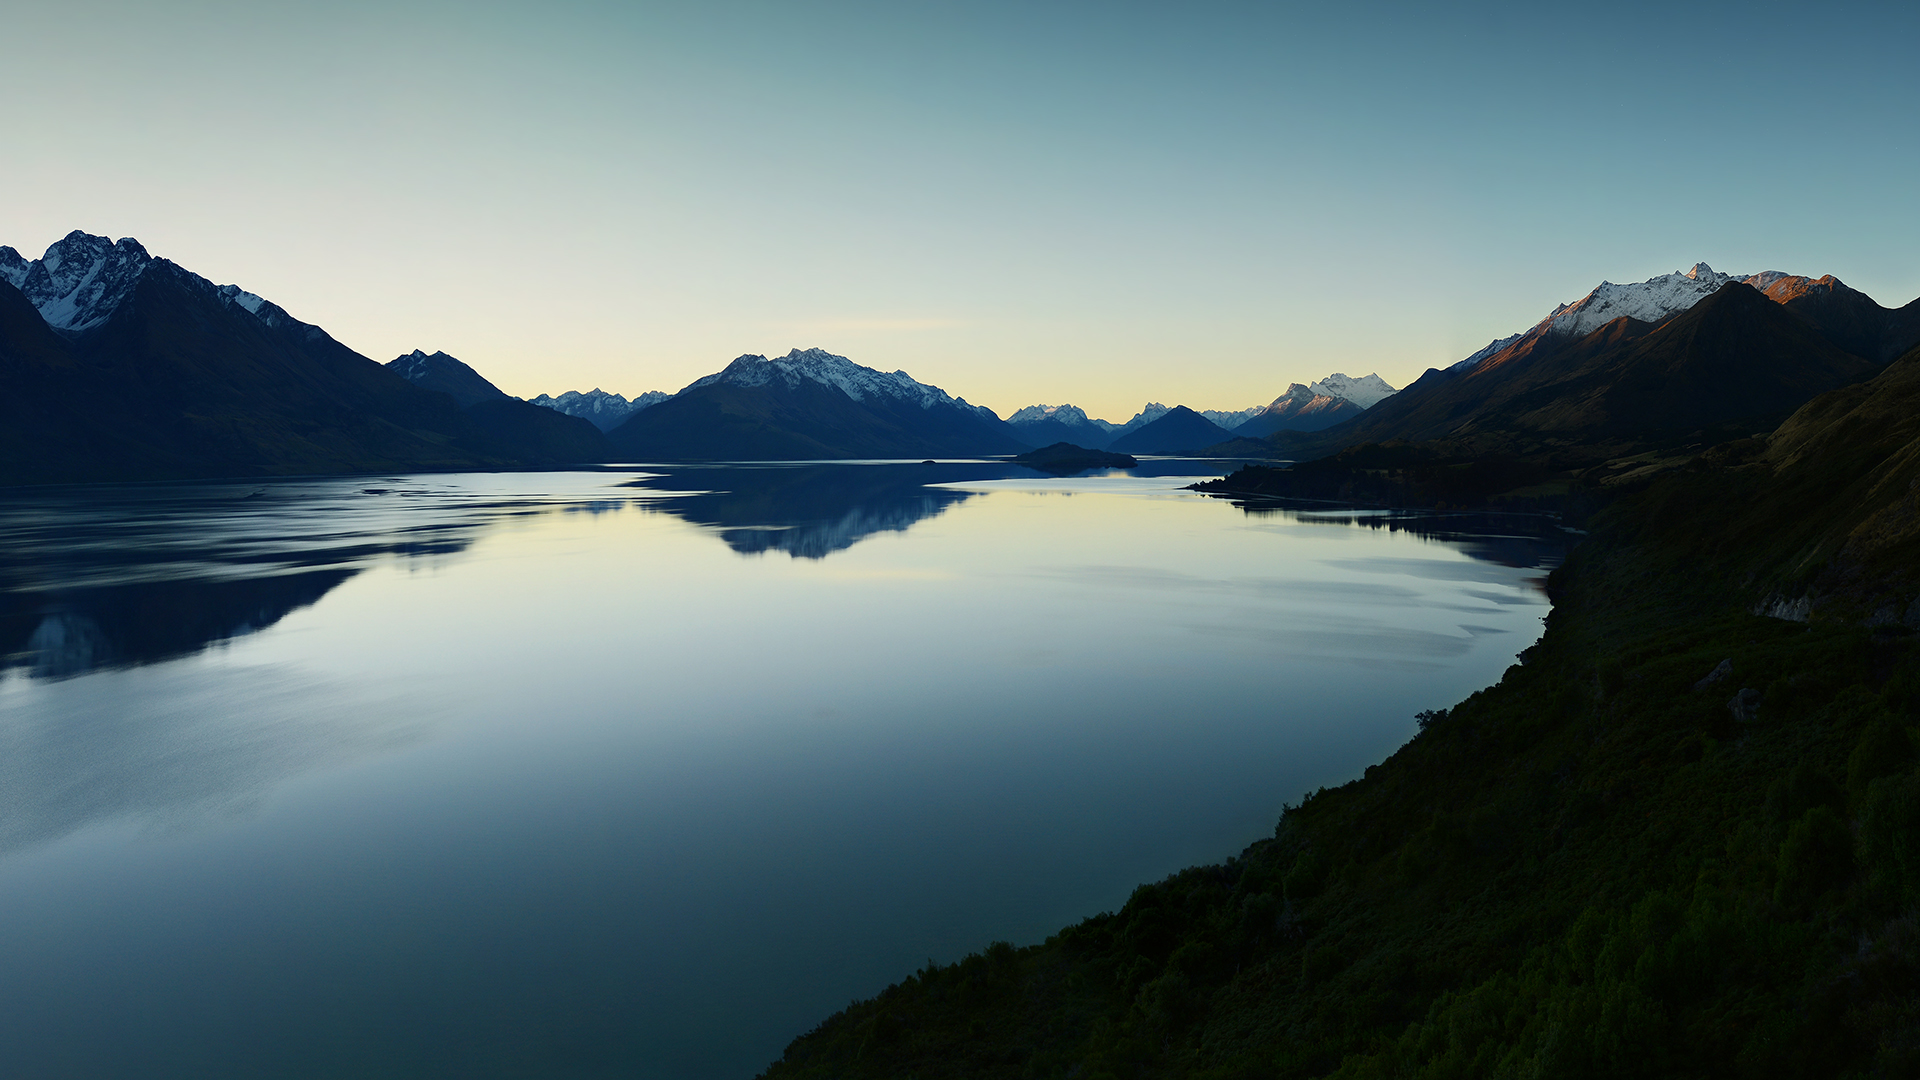
\includegraphics[width=.4\textwidth]{template2.jpg}}\hspace{20pt}
	\subfloat[待规定化图片2的彩色分布直方图]{
		\label{fig:2histogram}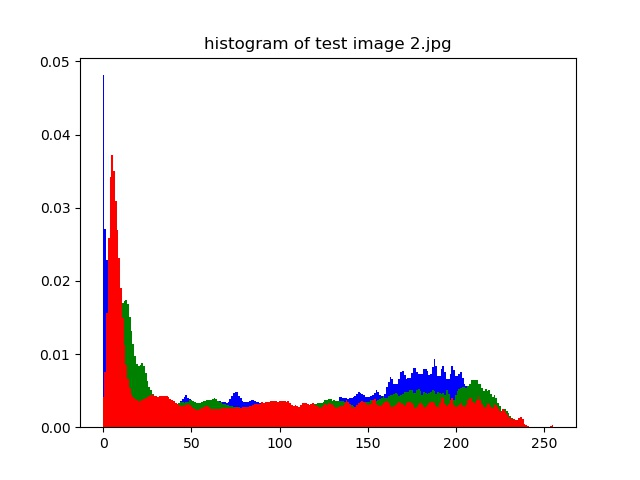
\includegraphics[scale=.3]{histogramoftestimage2.jpg}}
	\\
	\subfloat[待规定化图片3]{
		\label{fig:3}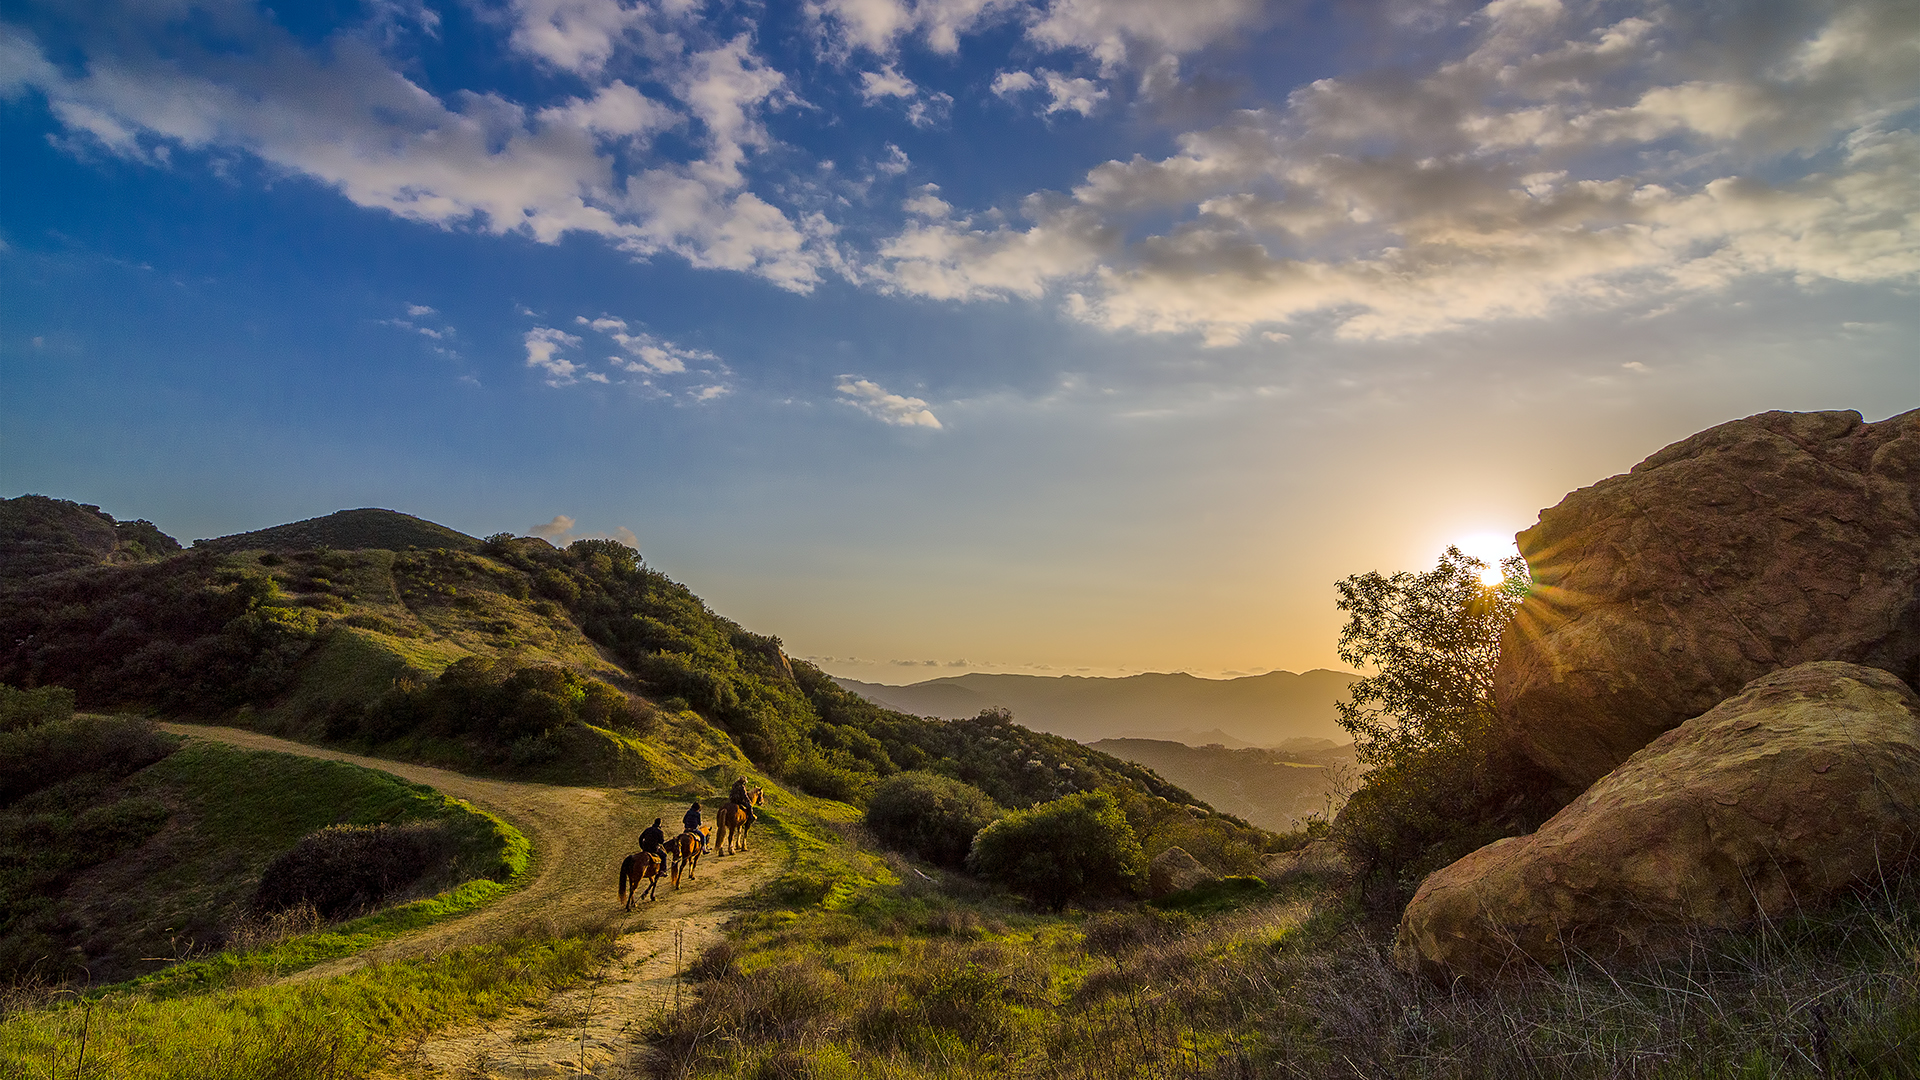
\includegraphics[width=.4\textwidth]{template3.jpg}}\hspace{20pt}
	\subfloat[待规定化图片3的彩色分布直方图]{
		\label{fig:3histogram}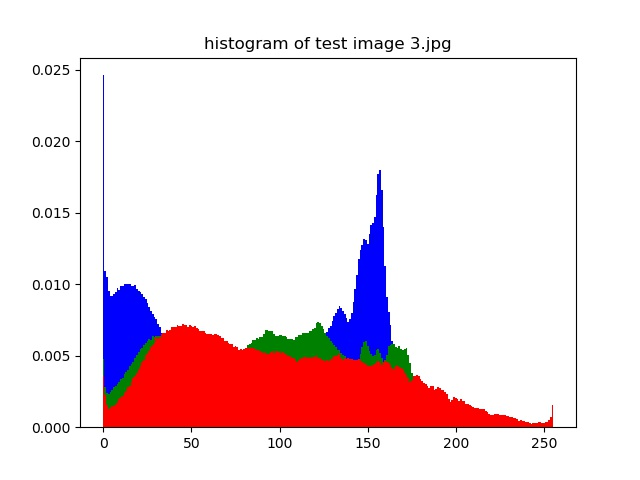
\includegraphics[scale=.3]{histogramoftestimage3.jpg}}
	\caption{待规定化三幅图片及其彩色分布直方图}\label{fig:guidinghua}
\end{figure}

将三幅图片进行直方图规定化的结果和相应图片的彩色直方图如图(\ref{fig:guiguidinghua})所示。

\begin{figure}[htb]
	\centering
	\subfloat[规定化后图片1]{
		\label{fig:gui1}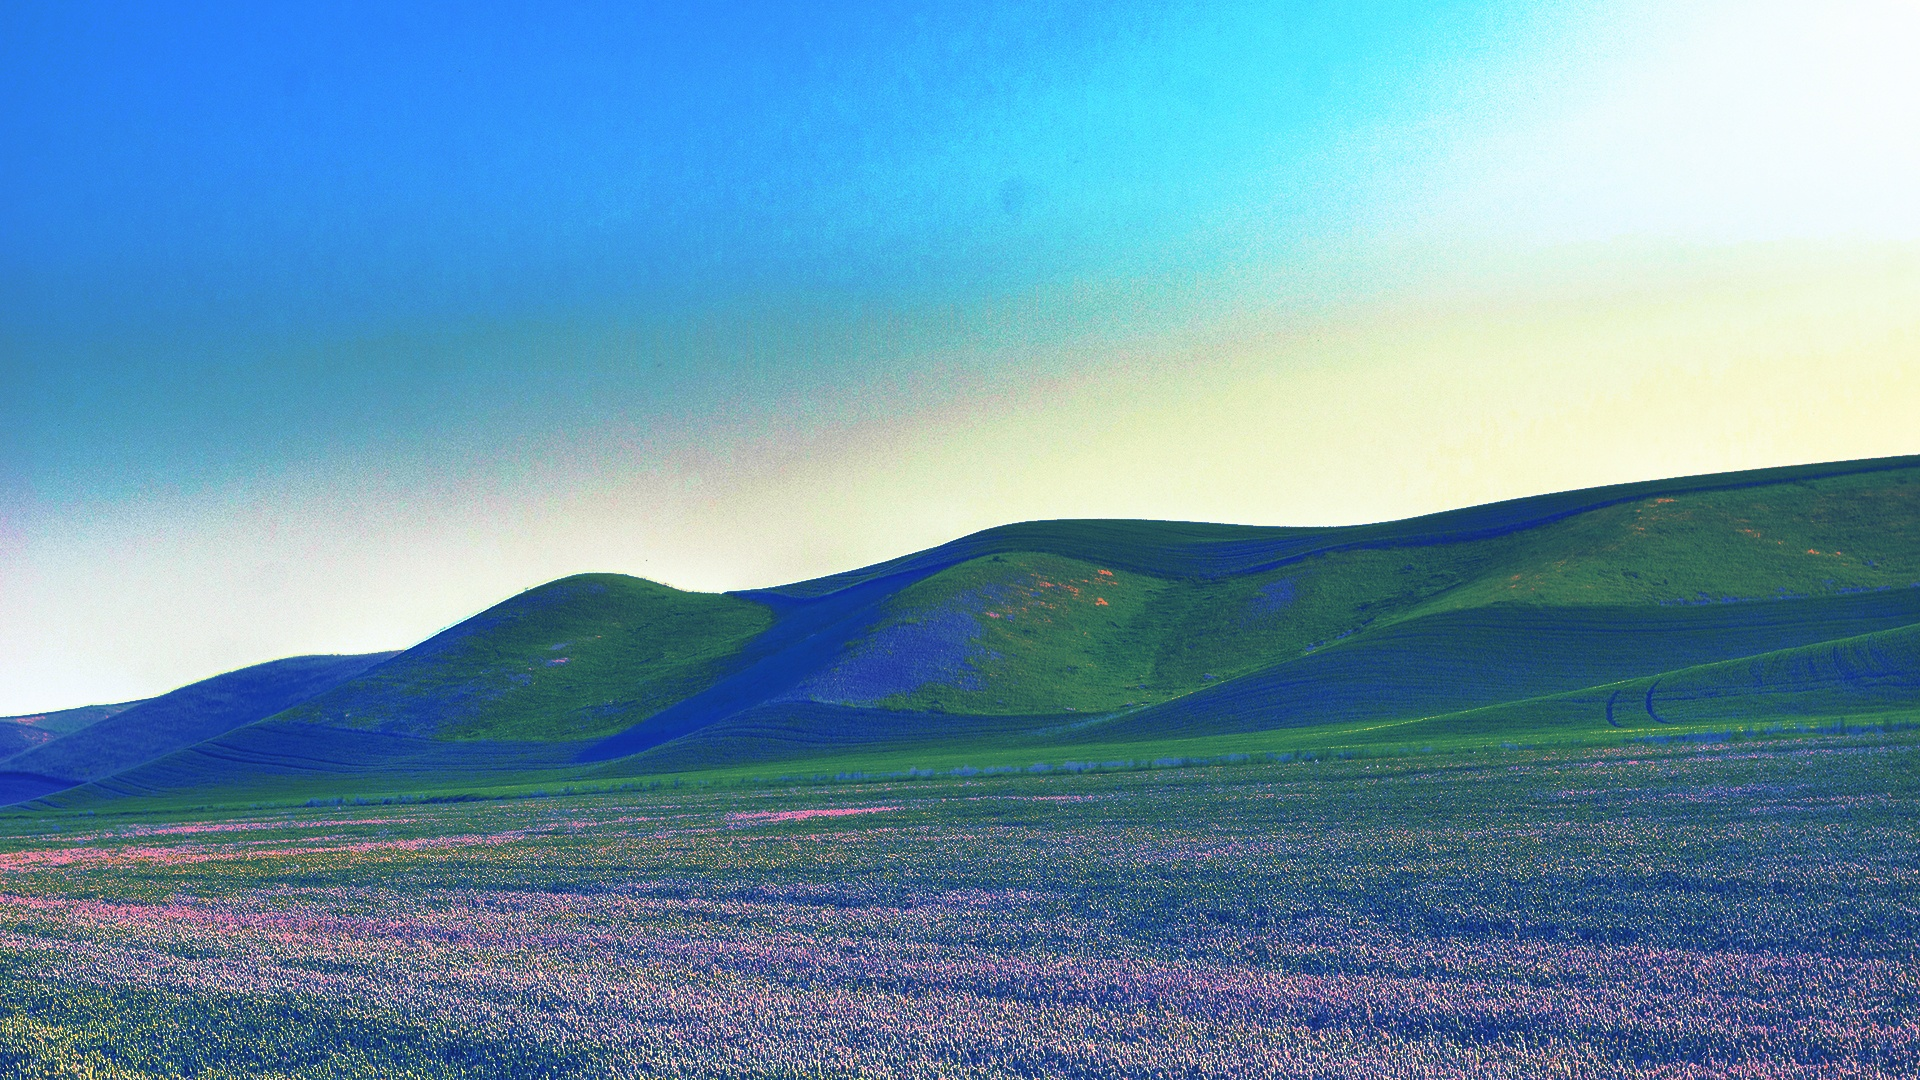
\includegraphics[width=.4\textwidth]{1.jpg}}\hspace{20pt}
	\subfloat[图片1规定化的彩色分布直方图]{
		\label{fig:gui1histogram}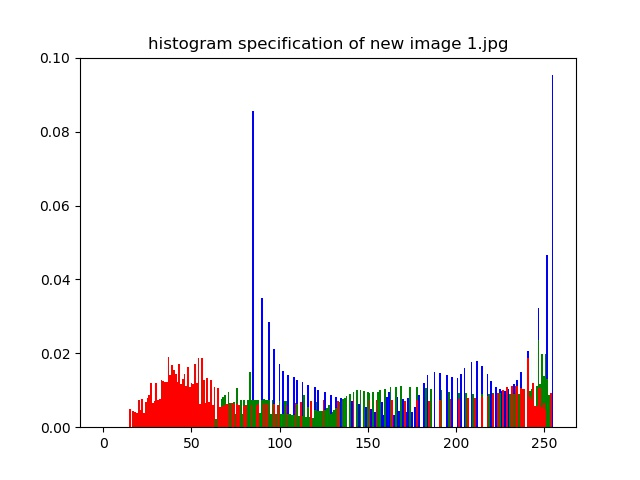
\includegraphics[scale=.3]{histogramspecificationofnewimage1.jpg}}
	\\
	\subfloat[规定化后图片2]{
		\label{fig:gui2}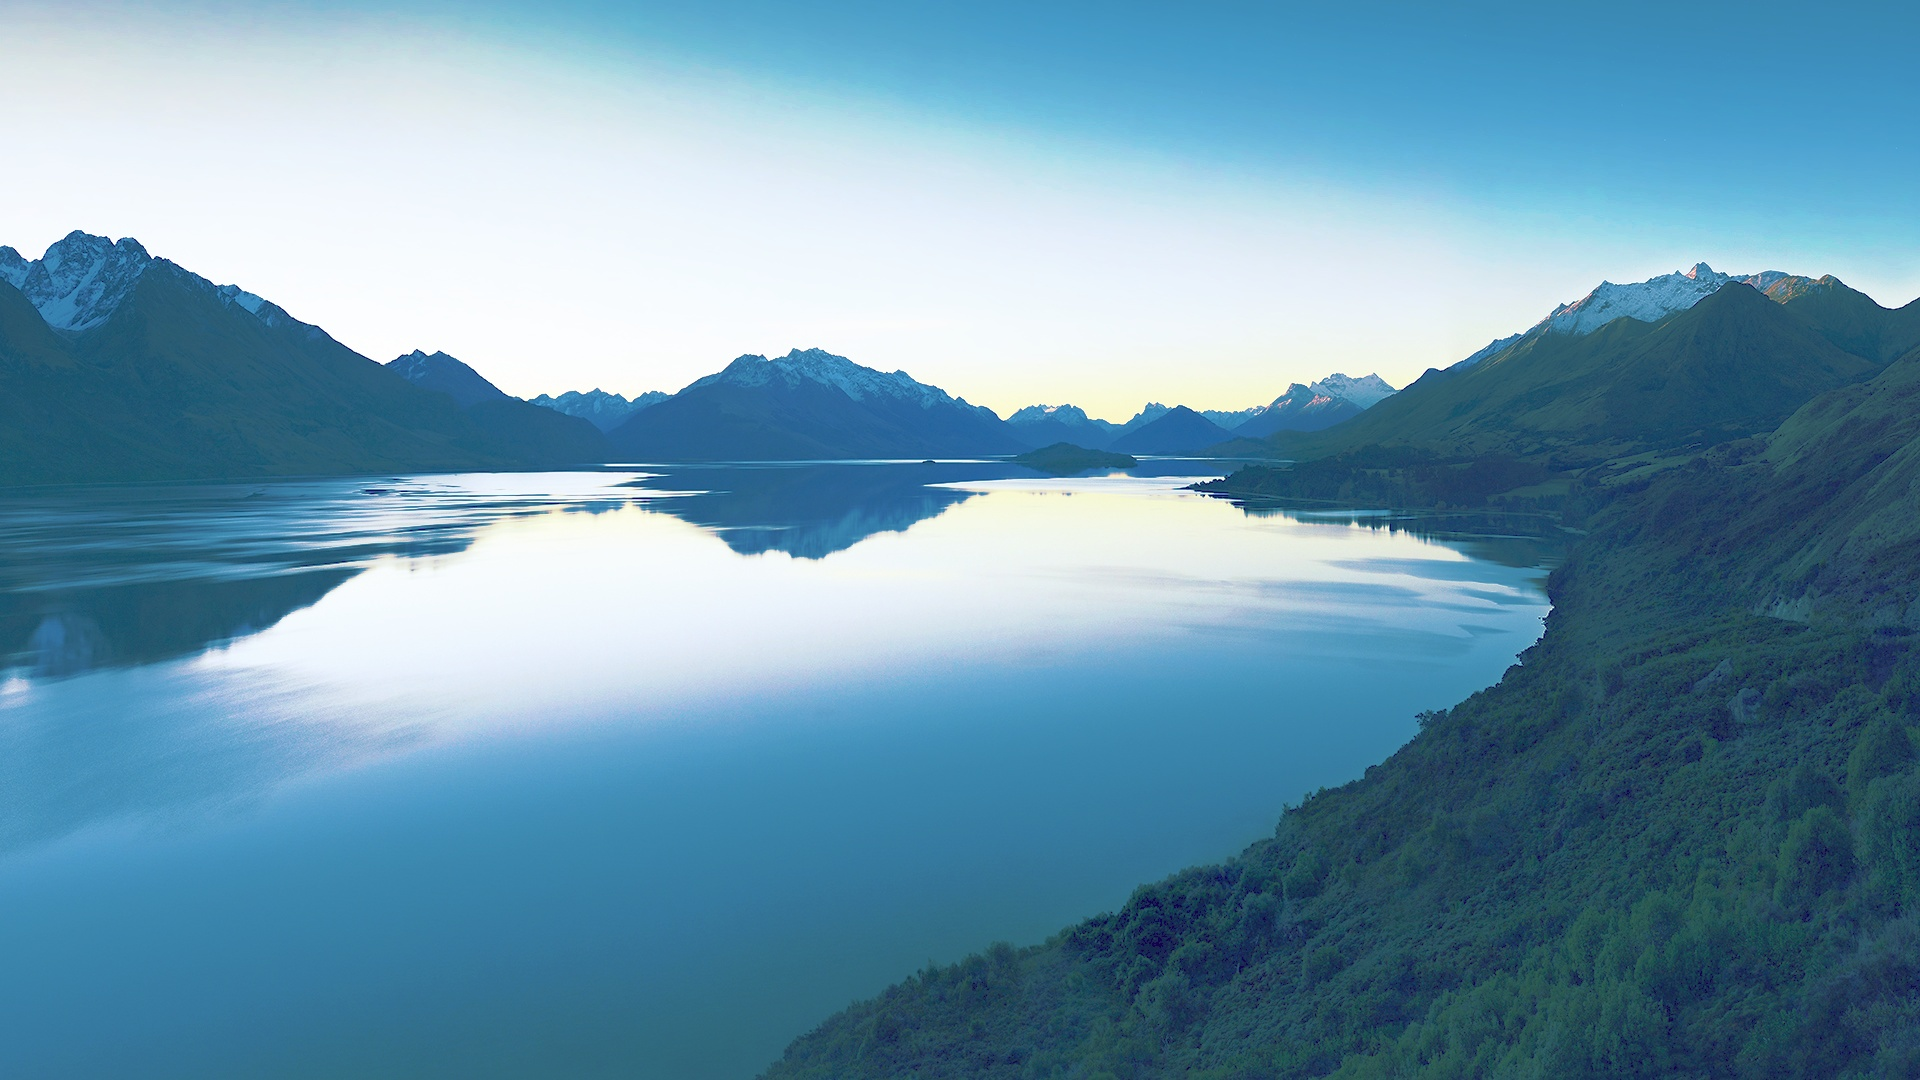
\includegraphics[width=.4\textwidth]{2.jpg}}\hspace{20pt}
	\subfloat[图片2规定化的彩色分布直方图]{
		\label{fig:gui2histogram}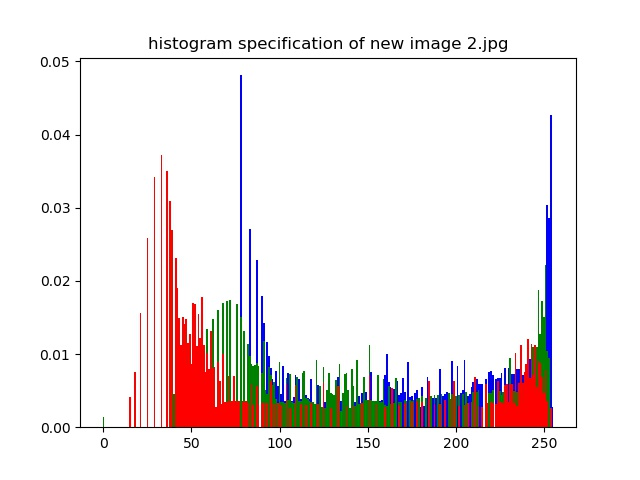
\includegraphics[scale=.3]{histogramspecificationofnewimage2.jpg}}
	\\
	\subfloat[规定化后图片3]{
		\label{fig:gui3}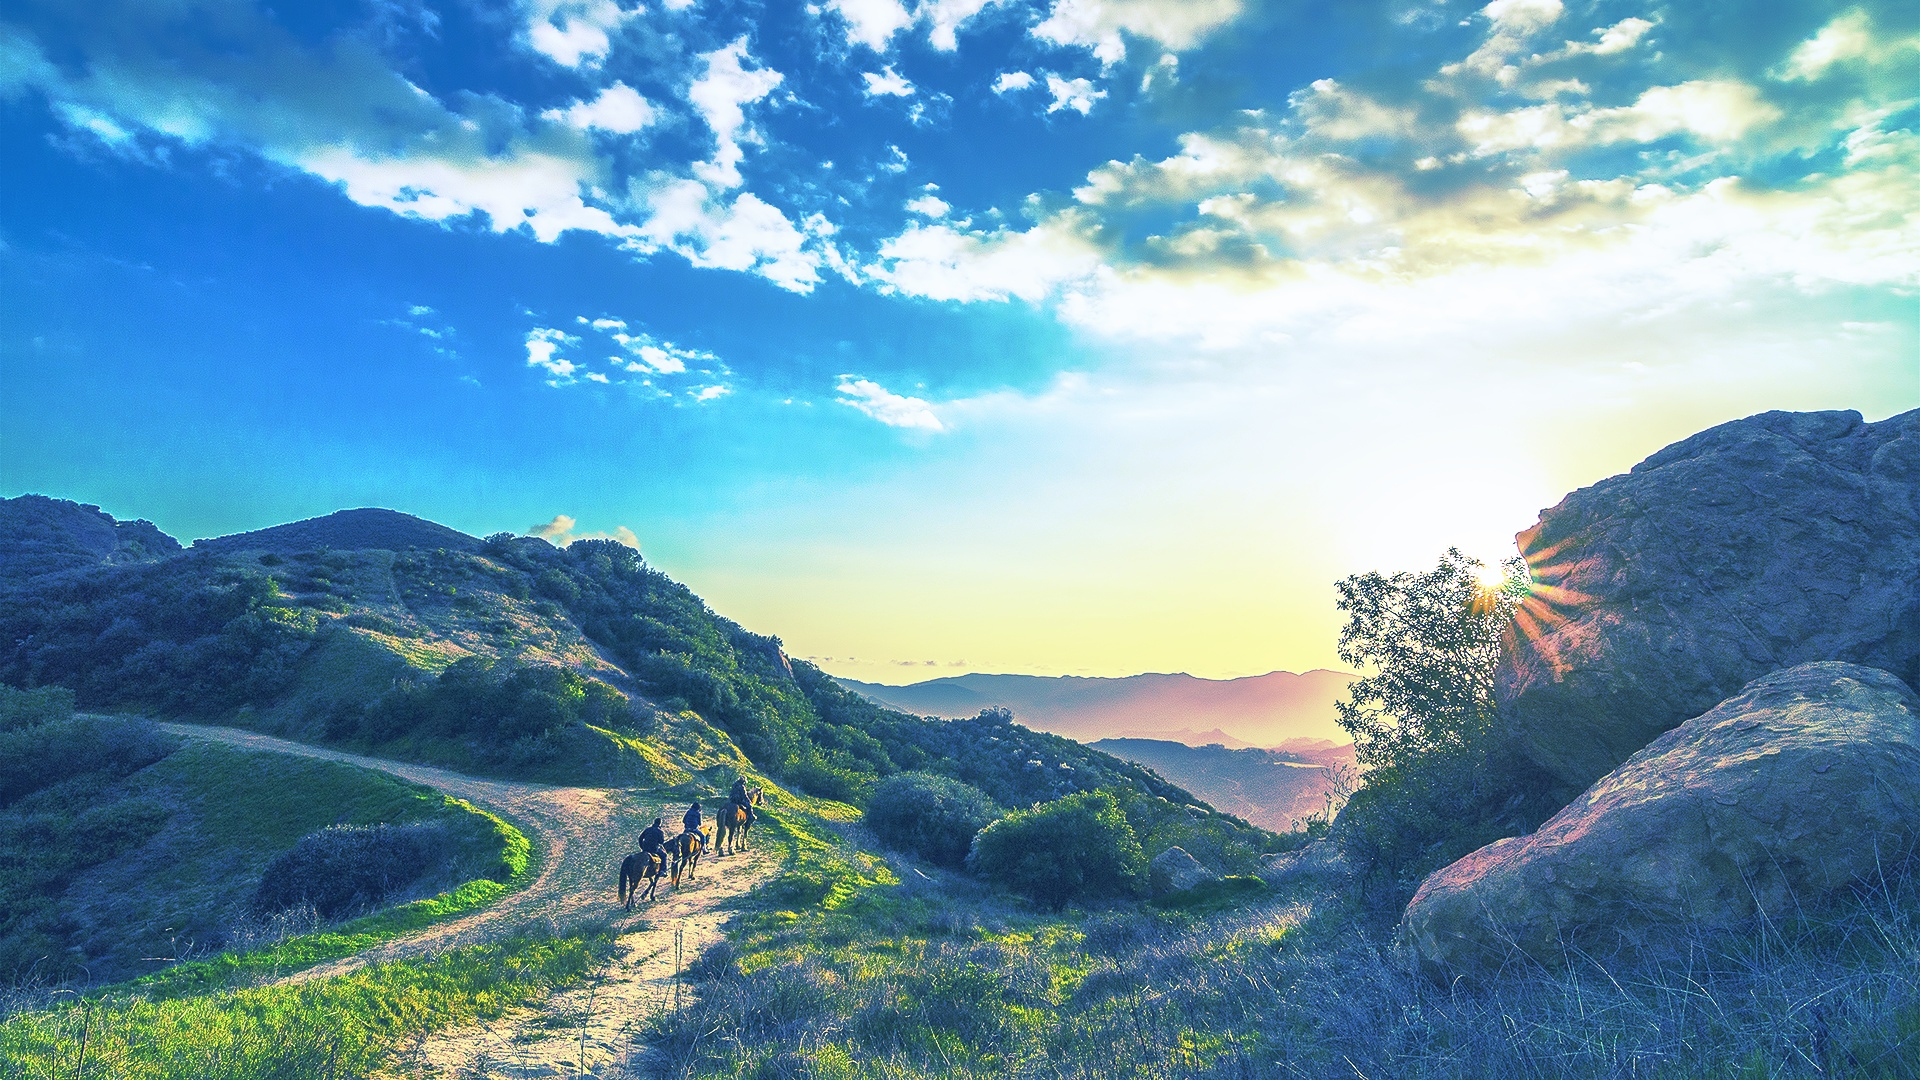
\includegraphics[width=.4\textwidth]{3.jpg}}\hspace{20pt}
	\subfloat[图片3规定化的彩色分布直方图]{
		\label{fig:gui3histogram}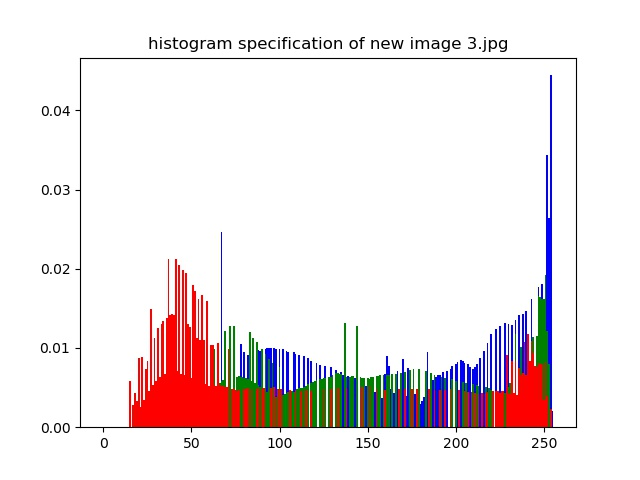
\includegraphics[scale=.3]{histogramspecificationofnewimage3.jpg}}
	\caption{规定化后三幅图片及其彩色分布直方图}\label{fig:guiguidinghua}
\end{figure}

可以看到,经过规定化后的图片如图(\ref{fig:gui1})(\ref{fig:gui2})(\ref{fig:gui3})所示,整体风格接近模板图片图(\ref{fig:template}),三幅图片经过规定化后的彩色分布直方图如图(\ref{fig:gui1histogram})(\ref{fig:gui2histogram})(\ref{fig:gui3histogram})所示,分布也接近模板图片的彩色分布图(\ref{fig:templatehistogram})。

\subsection{同态滤波}

同态滤波的原图是采用书上的示例图片,是一张光照分布不均匀的骨骼照片,如图(\ref{fig:bone})所示,使用章节\ref{sec:tongtailv}的算法,得到的结果如图(\ref{fig:tongtaibone})所示。

\begin{figure}[htb]
	\centering
	\subfloat[光照分布不均匀的骨骼照片]{
		\label{fig:bone}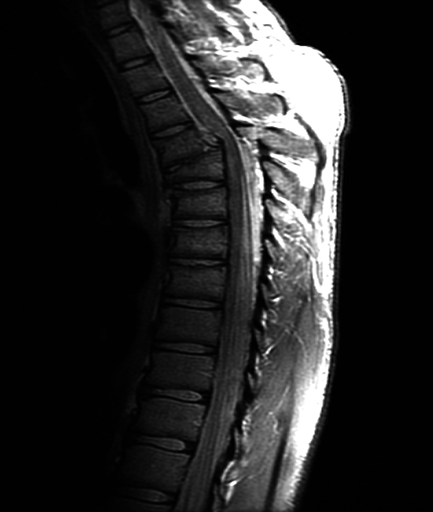
\includegraphics[width=.4\textwidth]{filter.png}}\hspace{20pt}
	\subfloat[经同态滤波的骨骼照片]{
		\label{fig:tongtaibone}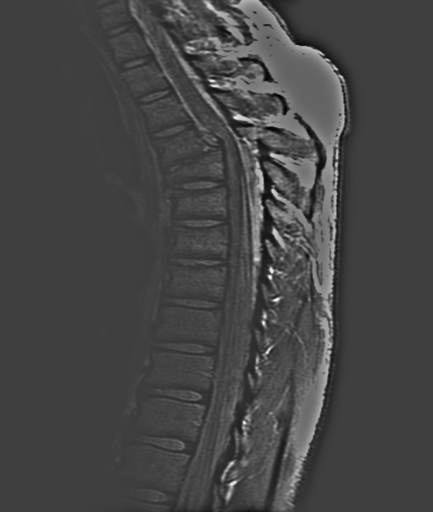
\includegraphics[width=.4\textwidth]{homomorphic_filter_result.png}}
	\caption{光照分布不均匀的骨骼照片及其同态滤波的结果}\label{fig:bone1}
\end{figure}

\subsection{双边滤波}

双边滤波采用的图片是lena的原图,如图(\ref{fig:lena1})所示,经过双边滤波后的结果如图(\ref{fig:shuanglena})所示。可以看见,面部和帽子处的细节变得平滑,但是边缘处又不发生模糊现象,是进过了双边滤波的结果。

\begin{figure}[htb]
	\centering
	\subfloat[lena原图]{
		\label{fig:lena1}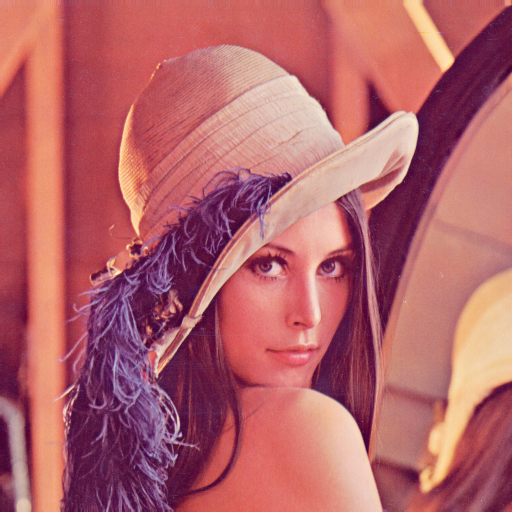
\includegraphics[width=.4\textwidth]{lena.png}}\hspace{20pt}
	\subfloat[经双边滤波的lena图]{
		\label{fig:shuanglena}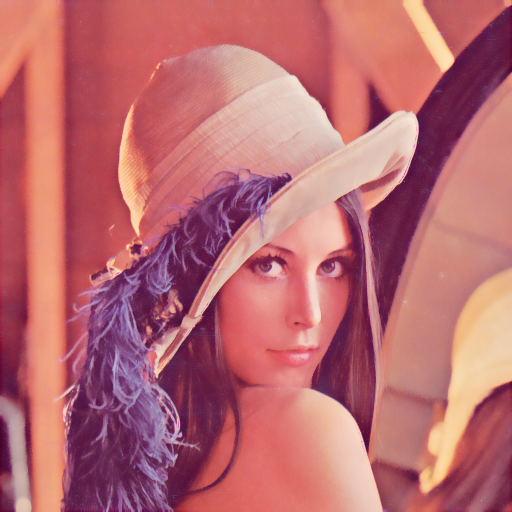
\includegraphics[width=.4\textwidth]{bilateral_filter.png}}
	\caption{lena原图和经过双边滤波后的结果}\label{fig:shuang}
\end{figure}



\section{实验结论}

\begin{enumerate}
\item 直方图均衡化可以使对比度不明显的图片对比度增强,从而达到显现更多细节的效果;
\item 直方图规定化可以使目标图片的直方图分布接近模板图片的直方图分布,简言之是一种“按照模板生成相应滤镜”的方法,获得与模板图片风格相近的图片。但是模板图片只有一张,直方图规定化之后的结果并不一定能较好的契合原图片;
\item 同态滤波是一种可以衰减图片低频分量、放大高频分量的频域滤波方法,可以进行动态范围的压缩和对比度增强;
\item 双边滤波不仅可以很好地滤除掉图像中随机出现的高斯噪声,还可以保留图片中的边缘细节,结合了高斯低通滤波和$\alpha$-截尾均值滤波各自的优点,也消除二者的缺点,是一种较好的非线性滤波算法,根据实验结果,双边滤波有“除雀斑”的功能。
\end{enumerate}

\renewcommand\refname{参考文献}
 
\begin{thebibliography}{1}
\bibitem{book:li}
Rafael C. Gonzalez \& Richard E. Woods (2020). Digital Image Processing (4th ed.).

\end{thebibliography}

\newpage
\begin{appendices}

\section{生成直方图--generate\_histogram.py}\label{app:gen}
\begin{lstlisting}[language=python]
import numpy as np
import matplotlib.pyplot as plt
from src.read_write_img import *


class Histogram(object):
    def __init__(self, img):
        self.img = img
        self.histogram = np.zeros(256, dtype=float)

    def generate_histogram(self):
        height, width = np.shape(self.img)
        for i in range(height):
            for j in range(width):
                # print(self.img[i, j])
                self.histogram[self.img[i, j]] += 1
        self.histogram = self.histogram / np.sum(self.histogram)
        return self.histogram

    def show_histogram(self, title, file_path, file_name, color='b'):
        plt.bar(range(len(self.histogram)), self.histogram, width=1, color=color)
        plt.title(title)
        plt.savefig(file_path + file_name + '.jpg')
        plt.show()


def main():
    img = read_source_img_with_gray_from_file()
    histogram = Histogram(img)
    _ = histogram.generate_histogram()
    title = 'histogram of source image'
    file_path = '../data/histogram_result/'
    histogram.show_histogram(title, file_path, title)


if __name__ == '__main__':
    main()

\end{lstlisting}

\section{直方图均衡化--histogram\_equalization.py}\label{app:hisequ}
\begin{lstlisting}[language=python]
from src.generate_histogram import *


class HistogramEqualization(object):
    def __init__(self, img):
        self.img = img
        self.img_hist = Histogram(img)
        self.img_histogram = self.img_hist.generate_histogram()
        self.img_hist.show_histogram("histogram of source image", '../data/histogram_result/',
                                     "histogram of source image")
        self.histogram_equal = np.zeros(256)
        self.histogram_spec = np.zeros(256)

    def histogram_equalization(self):
        self.histogram_equal = np.cumsum(self.img_histogram)
        height, width = np.shape(self.img)
        self.histogram_equal = np.uint8(255 * self.histogram_equal + 0.5)
        out_image = np.uint8(np.zeros((height, width)))
        for i in range(height):
            for j in range(width):
                out_image[i, j] = self.histogram_equal[self.img[i, j]]
        cv.imshow("histogram equalization", out_image)
        cv.waitKey(0)
        cv.destroyAllWindows()
        write_img_to_file(out_image, 'histogram_result/histogram equalization of source image')
        histogram = Histogram(out_image)
        chart = histogram.generate_histogram()
        histogram.show_histogram("histogram equalization of source image", '../data/histogram_result/',
                                 "histogram equalization of source image")


def main():
    img = read_source_img_with_gray_from_file()
    ht = HistogramEqualization(img)
    ht.histogram_equalization()


if __name__ == '__main__':
    main()

\end{lstlisting}

\section{直方图规定化--histogram\_specification.py}\label{app:hisspec}
\begin{lstlisting}[language=python]
from src.read_write_img import *
from src.generate_histogram import *
import matplotlib.pyplot as plt
import os


class HistogramSpecification(object):
    def __init__(self, template_img):
        self.template_img = template_img
        self.img_b, self.img_g, self.img_r = cv.split(self.template_img)
        self.histogram_b = Histogram(self.img_b).generate_histogram()
        self.histogram_g = Histogram(self.img_g).generate_histogram()
        self.histogram_r = Histogram(self.img_r).generate_histogram()
        self.generate_histogram('../data/histogram_result/', 'histogram of template image',
                                'histogram of template image')
        self.histogram_reverse_b = self.calculate_reverse_mapping(
            np.uint8((256 - 1) * np.cumsum(self.histogram_b) + 0.5))
        self.histogram_reverse_g = self.calculate_reverse_mapping(
            np.uint8((256 - 1) * np.cumsum(self.histogram_g) + 0.5))
        self.histogram_reverse_r = self.calculate_reverse_mapping(
            np.uint8((256 - 1) * np.cumsum(self.histogram_r) + 0.5))
        self.target_b = None
        self.target_g = None
        self.target_r = None
        self.template2target_b = None
        self.template2target_g = None
        self.template2target_r = None

    @staticmethod
    def calculate_reverse_mapping(histogram):
        mapping = list(histogram)
        off_mapping = []
        pre_f = 0.0
        for i in range(256):
            try:
                temp_f = mapping.index(i)
                pre_f = temp_f
            except ValueError:
                temp_f = pre_f
            off_mapping.append(temp_f)
        off_mapping = np.array(off_mapping)
        # plt.bar(range(len(off_mapping)), off_mapping, width=1)
        # plt.title("reverse mapping")
        # plt.show()
        return off_mapping

    def generate_new_image(self, target_img, file):
        self.target_b, self.target_g, self.target_r = cv.split(target_img)

        histogram_b = Histogram(self.target_b)
        histogram_g = Histogram(self.target_g)
        histogram_r = Histogram(self.target_r)
        target_histogram_b = histogram_b.generate_histogram()
        target_histogram_g = histogram_g.generate_histogram()
        target_histogram_r = histogram_r.generate_histogram()

        plt.bar(range(len(target_histogram_b)), target_histogram_b, width=1, color='b')
        plt.bar(range(len(target_histogram_g)), target_histogram_g, width=1, color='g')
        plt.bar(range(len(target_histogram_r)), target_histogram_r, width=1, color='r')
        plt.title('histogram of test image ' + str(file))
        plt.savefig('../data/histogram_result/' + 'histogram of test image ' + str(file) + '.jpg')
        plt.show()

        target_histogram_b = np.uint8((256 - 1) * np.cumsum(target_histogram_b) + 0.5)
        target_histogram_g = np.uint8((256 - 1) * np.cumsum(target_histogram_g) + 0.5)
        target_histogram_r = np.uint8((256 - 1) * np.cumsum(target_histogram_r) + 0.5)
        self.template2target_b = self.calculate_target_mapping(target_histogram_b, self.histogram_reverse_b)
        self.template2target_g = self.calculate_target_mapping(target_histogram_g, self.histogram_reverse_g)
        self.template2target_r = self.calculate_target_mapping(target_histogram_r, self.histogram_reverse_r)
        return self.generate_new_image_from_template(file)

    @staticmethod
    def calculate_target_mapping(target_histogram, template_histogram):
        target_map = list(target_histogram)
        template_map = list(template_histogram)
        final_map = []
        for i in range(256):
            temp_tar = target_map[i]
            temp_tem = template_map[temp_tar]
            final_map.append(temp_tem)
        final_map = np.array(final_map)
        return final_map

    def generate_new_image_from_template(self, file):
        height, width = np.shape(self.target_b)
        # print(height, width)
        for i in range(height):
            for j in range(width):
                temp_b = self.target_b[i, j]
                self.target_b[i, j] = self.template2target_b[temp_b]
                temp_g = self.target_g[i, j]
                self.target_g[i, j] = self.template2target_g[temp_g]
                temp_r = self.target_r[i, j]
                self.target_r[i, j] = self.template2target_r[temp_r]
        new_img = cv.merge([self.target_b, self.target_g, self.target_r])
        histogram_b = Histogram(self.target_b)
        histogram_g = Histogram(self.target_g)
        histogram_r = Histogram(self.target_r)
        chart_b = histogram_b.generate_histogram()
        chart_g = histogram_g.generate_histogram()
        chart_r = histogram_r.generate_histogram()

        plt.bar(range(len(chart_b)), chart_b, width=1, color='b')
        plt.bar(range(len(chart_g)), chart_g, width=1, color='g')
        plt.bar(range(len(chart_r)), chart_r, width=1, color='r')
        plt.title('histogram specification of new image ' + str(file))
        plt.savefig('../data/histogram_result/' + 'histogram specification of new image ' + str(file) + '.jpg')
        plt.show()

        return new_img

    def generate_histogram(self, file_path, file_name, title):
        plt.bar(range(len(self.histogram_b)), self.histogram_b, width=1, color='b')
        plt.bar(range(len(self.histogram_g)), self.histogram_g, width=1, color='g')
        plt.bar(range(len(self.histogram_r)), self.histogram_r, width=1, color='r')
        plt.title(title)
        plt.savefig(file_path + file_name + '.jpg')
        plt.show()


def main():
    template_img = read_template_img_rgb_from_file()
    hs = HistogramSpecification(template_img)
    test_path = '../data/test/'
    output_path = '../data/histogram_result/'
    img_list = os.listdir(test_path)
    for file in img_list:
        img_path = os.path.join(test_path, file)
        print('open image ' + str(img_path))
        target_img = cv.imread(img_path)
        result_img = hs.generate_new_image(target_img, file)
        print('finish change ' + str(file))
        output_path_file = os.path.join(output_path, file)
        print(output_path_file)
        show_img(result_img, 'histogram specification of image ' + str(file))
        cv.imwrite(output_path_file, result_img)


if __name__ == '__main__':
    main()

\end{lstlisting}

\section{同态滤波--homomorphic\_filter.py}\label{app:homo}
\begin{lstlisting}[language=python]
import matplotlib.pyplot as plt
from src.read_write_img import *
from src.fast_fourier_transform import *


class HomomorphicFilter(object):
    def __init__(self, img, a=1.0, b=1.5):
        self.img = img
        self.fft_img = None
        self.filter_result = None
        self.ifft_img = None
        self.a = float(a)
        self.b = float(b)
        self.height, self.width = np.shape(img)

    def homomorphic_filter(self):
        self.generate_fft_img()
        print("finish fft image")
        result = self.gaussian_filter()
        print("finish filter image")
        return result

    def gaussian_filter(self):
        M = self.height
        N = self.width
        sigma = 10
        (X, Y) = np.meshgrid(np.linspace(0, N - 1, N), np.linspace(0, M - 1, M))
        center_x = np.ceil(N / 2)
        center_y = np.ceil(M / 2)
        gauss_filter_matrix = np.square(X - center_x) + np.square(Y - center_y)

        loss_pass = np.exp(-gauss_filter_matrix / (2 * sigma * sigma))
        high_pass = 1 - loss_pass
        loss_pass_shift = np.fft.ifftshift(loss_pass.copy())
        # show_img(loss_pass_shift, "sdgdf")
        high_pass_shift = np.fft.ifftshift(high_pass.copy())

        img_out_low = np.real(my_ifft(self.fft_img.copy() * loss_pass_shift))
        # show_img(img_out_low, "sdf")
        img_out_high = np.real(my_ifft(self.fft_img.copy() * high_pass_shift))
        # show_img(img_out_high, "sdf2")

        gamma1 = 0.3
        gamma2 = 1.5

        img_out = gamma1 * img_out_low[0:self.height, 0:self.width] + gamma2 * img_out_high[0:self.height, 0:self.width]

        self.filter_result = img_out
        # show_img(img_out, "img_out")

        img_hmf = np.expm1(img_out)
        # show_img(img_hmf, "Ihmf")
        print("min img_hmf {}, max img_hmf {}", np.min(img_hmf), np.max(img_hmf))
        img_hmf = (img_hmf - (-354) * np.min(img_hmf)) / (0.915 * np.max(img_hmf) - (-354) * np.min(img_hmf))
        img_result = np.array(255 * img_hmf, dtype="uint8")
        # show_img(img_result, "img_result")
        return img_result

    def generate_fft_img(self):
        img_log = np.log1p(np.array(self.img, dtype="float") / 255)
        self.fft_img = my_fft(img_log)
        show_img(np.real(self.fft_img), "sdfsdfd")


def main():
    img = read_homomorphic_filter()
    # img = cv.resize(img, (512, 512), interpolation=cv.INTER_NEAREST)
    my_fft = HomomorphicFilter(img)
    result = my_fft.homomorphic_filter()
    show_img(result, 'homomorphic filter')
    write_img_to_file(result, 'filter_result/' + 'homomorphic_filter_result')


if __name__ == '__main__':
    main()

\end{lstlisting}

\section{快速傅里叶变换和快速傅里叶反变换--fast\_fourier\_transform.py}\label{app:fft}
\begin{lstlisting}[language=python]
import numpy as np


def my_fft(img):
    print('start to fft')
    height, width = np.shape(img)
    result_complex = img.astype(np.complex)

    def fft_one(a):
        len = a.size
        if len == 1:
            return
        a0 = np.zeros(len // 2, complex)
        a1 = np.zeros(len // 2, complex)
        for i in range(0, len, 2):
            a0[i // 2] = a[i]
            a1[i // 2] = a[i + 1]
        fft_one(a0)
        fft_one(a1)

        wn = complex(np.cos(2 * np.pi / len), np.sin(2 * np.pi / len))
        w = complex(1, 0)
        for i in range(len // 2):
            t = w * a1[i]
            a[i] = a0[i] + t
            a[i + len // 2] = a0[i] - t
            w = w * wn

    for i in range(height):
        fft_one(result_complex[i])
    for i in range(width):
        fft_one(result_complex[:, i])

    print('finish fft')
    return result_complex


def my_ifft(img):
    print('start to ifft')
    height, width = np.shape(img)

    result_complex = img.astype(np.complex)
    result = np.zeros([height, width], np.float64)

    def ifft_one(a):
        len = a.size
        if len == 1:
            return

        a0 = np.zeros(len // 2, complex)
        a1 = np.zeros(len // 2, complex)
        for i in range(0, len, 2):
            a0[i // 2] = a[i]
            a1[i // 2] = a[i + 1]
        ifft_one(a0)
        ifft_one(a1)

        wn = complex(np.cos(2 * np.pi / len), -1 * np.sin(2 * np.pi / len))  # 参数
        w = complex(1, 0)
        for i in range(len // 2):
            t = w * a1[i]
            a[i] = a0[i] + t
            a[i + len // 2] = a0[i] - t
            w = w * wn

    for i in range(height):
        ifft_one(result_complex[i])
    for i in range(width):
        ifft_one(result_complex[:, i])

    for i in range(height):
        for j in range(width):
            result[i, j] = np.abs(result_complex[i, j] / (height * width))

    print('finish ifft')
    return result



\end{lstlisting}

\section{双边滤波--bilateral\_filter.py}
\begin{lstlisting}[language=python]
import numpy as np
from src.read_write_img import *


class BilateralFilter(object):
    def __init__(self, img, radius, color_sigma, s_sigma):
        self.img = img
        self.img_b, self.img_g, self.img_r = cv.split(img)
        self.img_b_result, self.img_g_result, self.img_r_result = cv.split(img)
        self.height, self.width = np.shape(self.img_b)
        self.radius = radius
        self.color_sigma = color_sigma
        self.s_sigma = s_sigma
        self.weight_s_y = []
        self.weight_s_x = []
        self.weight_s = []
        self.color_weight = []
        self.k_max = 0
        self.generate_gauss_filter_template()

    def generate_gauss_filter_template(self):
        color_coe = -0.5 / np.square(self.color_sigma)
        for i in range(256):
            self.color_weight.append(np.exp(i ** 2 * color_coe))
        space_coe = -0.5 / np.square(self.s_sigma)
        for i in range(-self.radius, self.radius + 1):
            for j in range(-self.radius, self.radius + 1):
                r_sq = np.exp((np.square(i) + np.square(j)) * space_coe)
                self.weight_s_x.append(i)
                self.weight_s_y.append(j)
                self.weight_s.append(r_sq)
                self.k_max += 1

    def bilateral_filter_main(self, img):
        for i in range(self.height):
            for j in range(self.width):
                value = 0
                weight = 0
                for index in range(self.k_max):
                    print("i, j, index ", i, j, index)
                    temp_x = self.weight_s_x[index] + i
                    temp_y = self.weight_s_y[index] + j
                    if temp_x >= self.height or temp_y >= self.width or temp_x < 0 or temp_y < 0:
                        val = 0
                    else:
                        val = img[temp_x][temp_y]
                    temp_w = np.float32(self.weight_s[index]) * np.float32(self.color_weight[np.abs(val - img[i][j])])
                    value += val * temp_w
                    weight += temp_w
                img[i][j] = np.uint8(value / weight)
        return img

    def bilateral_filter(self):
        b_result = self.bilateral_filter_main(self.img_b_result)
        print('b_result', b_result)
        g_result = self.bilateral_filter_main(self.img_g_result)
        print('g_result', g_result)
        r_result = self.bilateral_filter_main(self.img_r_result)
        print('r_result', r_result)
        result_img = cv.merge([b_result, g_result, r_result])
        print(result_img)
        return result_img


def main():
    img = read_source_img_from_file()
    bf = BilateralFilter(img, 3, 30, 80)
    result = bf.bilateral_filter()
    show_img(result, 'bilateral filter')
    write_img_to_file(result, 'filter_result/bilateral_filter')


if __name__ == '__main__':
    main()

\end{lstlisting}



\section{读取图片和写回图片--}
\begin{lstlisting}[language=python]
import cv2 as cv


def read_source_img_from_file():
    file_path = '../data/lena512color.tiff'
    img = cv.imread(file_path)
    show_img(img, "Source image of lena")
    return img


def read_source_img_with_gray_from_file():
    file_path = '../data/lenagray.bmp'
    img = cv.imread(file_path, cv.IMREAD_GRAYSCALE)
    show_img(img, "Source image of lena")
    return img


def read_template_img_rgb_from_file():
    file_path = '../data/template1.jpg'
    img = cv.imread(file_path)
    show_img(img, "Template image")
    return img


def read_homomorphic_filter():
    file_path = '../data/filter2.tif'
    img = cv.imread(file_path, cv.IMREAD_GRAYSCALE)
    show_img(img, 'Source image to filter')
    return img


def write_img_to_file(img, file_name):
    file_path = '../data/' + file_name + '.png'
    cv.imwrite(file_path, img)


def show_img(img, title):
    cv.namedWindow(title, cv.WINDOW_FREERATIO)
    cv.imshow(title, img)
    cv.waitKey(0)
    cv.destroyAllWindows()


if __name__ == '__main__':
    read_source_img_from_file()
    # write_img_to_file()


\end{lstlisting}

\end{appendices}

\end{document}
